\section{State}

O padrão State permite alterar o comportamento de um objeto 
alterando seu estado interno. As operações que dependem do 
estado do objeto são definidas em uma interface conhecida 
pelo objeto, de forma que ele delegue essas operações 
para outra classe que implemente essa interface. 

Essa abordagem contribui para o reuso de operações 
que se repetem em classes relacionadas. Sem o State, 
essas classes teriam que ser instanciadas novamente 
a cada mudança de estado. Outra vantagem é que o 
padrão permite que o estado seja trocado dinamicamente 
durante a execução. A estrutura do padrão pode ser 
vista na figura \ref{state_struct}.

\begin{figure}[htb]
	\caption{\label{state_struct}Estrutura do State}
	\begin{center}
	    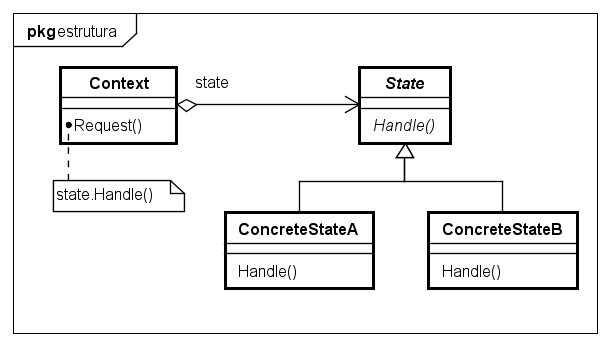
\includegraphics[scale=0.5]{5_padroes-contexto-funcional/5.3_comportamentais/5.3.08_state/state_estrutura.png}
	\end{center}
\end{figure}

\subsection*{Exemplo Orientado a Objetos}

Como exemplo, é considerada uma classe TCPConnection 
que define uma conexão de rede que pode estar em diversos 
estados: Estabelecida, escutando e fechada. Dependendo 
do estado em que a conexão se encontra, ela deve 
responder de forma diferente às operações que uma 
conexão TCP pode realizar. O padrão Strategy, cuja 
implementação pode ser vista no diagrama da imagem 
\ref{state_exemplo} e no código \ref{oostate}, é 
utilizado para encapsular em classes diferentes as 
operações referentes a cada estado da conexão. 
Dessa forma, a classe TCPConnection delega a uma classe 
que implementa a interface TCPState a execução das 
operações necessárias. Quando o estado interno da classe 
for modificado, a operação referente ao novo estado 
também será alterada automaticamente.

\begin{figure}[htb]
	\caption{\label{state_exemplo}Exemplo de State}
	\begin{center}
	    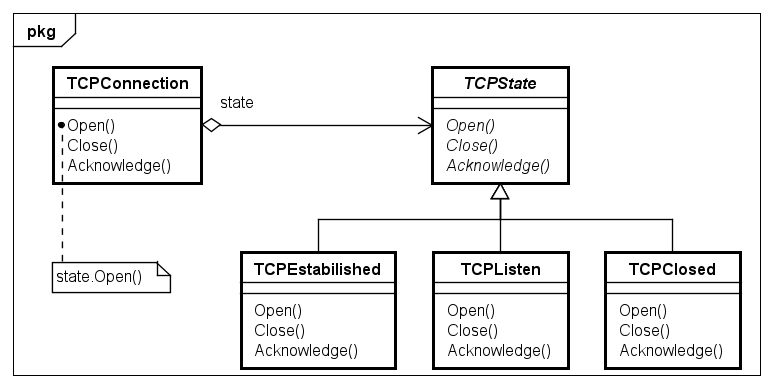
\includegraphics[scale=0.5]{5_padroes-contexto-funcional/5.3_comportamentais/5.3.08_state/state_exemplo.png}
	\end{center}
\end{figure}

\begin{lstlisting}[caption={State Orientação a Objetos},label=oostate]

class TCPConnection(var state : TCPState) {
  def Open(): Unit = state.Open()
  def Close(): Unit = state.Close()
  def Acknowledge(): Unit = state.Acknowledge()
}

trait TCPState {
  def Open()
  def Close()
  def Acknowledge()
}

class TCPEstabilished extends TCPState {
  def Open():Unit = {
    //Implementação para conexão estabelecida
  }
  def Close(): Unit = {
    //Implementação para conexão estabelecida
  }
  def Acknowledge(): Unit = {
    //Implementação para conexão estabelecida
  }
}

class TCPListen extends TCPState {
  def Open():Unit = {
    //Implementação para conexão escutando
  }
  def Close(): Unit = {
    //Implementação para conexão escutando
  }
  def Acknowledge(): Unit = {
    //Implementação para conexão escutando
  }
}

class TCPClosed extends TCPState {
  def Open():Unit = {
    //Implementação para conexão fechada
  }
  def Close(): Unit = {
    //Implementação para conexão fechada
  }
  def Acknowledge(): Unit = {
    //Implementação para conexão fechada
  }
}

\end{lstlisting}

\subsection*{Contexto Funcional}

\begin{comment}
Normalmente, a primeira alternativa que se tem em mente é 
o monad State. Porém, esse monad é focado em comportamentos 
que alteram o estado atual do nosso valor. Por mais que isso 
seja possível através do padrão State, por definição, sua 
intenção é fornecer comportamentos que não necessariamente 
altera o estado interno do valor.

Dessa forma, uma maneira interessante de definir o State 
no contexto funcional é utilizando uma case class que armazena, 
além dos valores comuns, um valor referente a um State. 
Esse State nada mais é do que outra clase class que 
irá armazenar, através de funções, os comportamentos que 
dependem de um estado. Da mesma forma que uma interface 
define as assinaturas das operações no exemplo orientado a 
objetos, aqui a definição da case class definirá que tipos 
de comportamentos a case class principal deverá possuir.

\begin{lstlisting}[caption={State Funcional},label=fpstate]
    
type TCPState = (() => Unit,
                 () => Unit,
                 () => Unit)

def Open(state : TCPState) : Unit = state._1()

def Close(state : TCPState) : Unit = state._2()

def Acknowledge(state : TCPState) : Unit = state._3()
    
\end{lstlisting}



\begin{lstlisting}[caption={State Funcional},label=fpstate]
    
val TCPEstabilished = (
  () => {
    //Operação Open para conexão estabelecida
  },
  () => {
    //Operação Close para conexão estabelecida
  },
  () => {
    //Operação Acknowledge para conexão estabelecida
  }
)

val TCPClosed = (
  () => {
    //Operação Open para conexão fechada
  },
  () => {
    //Operação Close para conexão fechada
  },
  () => {
    //Operação Acknowledge para conexão fechada
  }
)

val TCPListen = (
  () => {
    //Operação Open para conexão escutando
  },
  () => {
    //Operação Close para conexão escutando
  },
  () => {
    //Operação Acknowledge para conexão escutando
  }
)
    
\end{lstlisting}

É importante notar que, aqui, quando o estado do valor 
principal precisa ser supostamente modificado, o que na 
verdade acontecerá é que a função da case class State 
irá retornar o nosso valor atualizado.

\end{comment}